\subsection{Merkle Trees}
Consider a set $S = \{s_1, s_2, \cdots, s_n\}$ of strings
$s_i \in \{0, 1\}^*$. At some initial time, this set is compressed into a
\emph{root} string $s$ which is short ($|s| = \lambda$). This compressed string
is produced honestly and is given to a party called the \emph{verifier}. Given
this short trusted root string, the verifier receives claims from untrusted
\emph{provers} which claim that a certain piece of data $e$ existed in $S$.
The verifier's job is to decide whether such claims are truthful or fraudulent.

This protocol is an \emph{authenticated data structure}. It consists of
four algorithms $\mathcal{G}$, $\textsc{compress}$, $\textsc{prove}$,
$\textsc{verify}$. At the beginning of the execution, $\mathcal{G}(1^\lambda)$
is invoked to initialize the protocol parameters. These parameters can be shared
among multiple invocations of the protocol. As these parameters are fixed by the
protocol in its concrete implementations, we will make them implicit from now
on. A set $S$ is compressed by invoking $\textsc{compress}(S)$
which produces the root $s$. When an honest prover wishes to prove that some
element $e$ exists in $S$, they produce an \emph{inclusion proof} $\pi =
\textsc{prove}(S, e)$. When the verifier receives an element $e$ together
with a proof of inclusion $\pi$, they check its veracity by invoking
$\textsc{verify}(\pi, e, s)$, which returns $\true$ or $\false$.

Authenticated data structure protocols must be correct. This means that honest
executions should always work.

\begin{definition}[Correctness]
  Consider an authenticated data structure protocol
  $\Pi = (\textsc{compress}, \textsc{prove}, \textsc{verify})$.
  We say that $\Pi$ is
  \emph{correct} if

  \[\forall S:
    \forall e \in S:
    \textsc{verify}(\textsc{prove}(S, e), e, \textsc{compress}(S))\,.\]
\end{definition}

Such protocols are useful when $s$ and $\pi$ are short.

\begin{definition}[Succinctness]
  Consider an authenticated data structure protocol
  $\Pi = (\textsc{compress}, \textsc{prove}, \textsc{verify})$.
  We say that $\Pi$ is
  \emph{succinct} if
  for all $S$ it holds that

  \[|\textsc{compress}(S)| \in \bigO(polylog(|S|))
    \land
    \forall e \in S:
    |\textsc{prove}(S, e)| \in \bigO(polylog(|S|))
    \,.\]
\end{definition}

In the protocols we will explore, we will have $|s| = \lambda \in \bigO(1)$ and
$\pi \in \bigO(\log(|S|))$. Furthermore, $|S|$ will be polynomial in $\lambda$.

An authenticated data structure protocol is \emph{secure} if no adversary can
convince a verifier about the inclusion of an element which is not in the
set. This is made formal in the game illustrated in
Algorithm~\ref{alg.authenticated}.

\begin{figure}[t]
\begin{algorithm}[H]
    \caption{\label{alg.authenticated} The authenticated data structure challenger.}
    \begin{algorithmic}[1]
        \Function{\sf AUTH$_{\Pi,\mathcal{A}}$}{$\lambda$}
            \Let{(S, s_i, \pi)}{\mathcal{A}(1^\lambda)}
            \State\Return{$s_i \not\in S \land \textsc{verify}(\textsc{compress}(S), s_i, \pi)$}
        \EndFunction
        \vskip8pt
    \end{algorithmic}
\end{algorithm}
\end{figure}


\begin{definition}[Security]
  An authenticated data structure protocol $\Pi = (\textsc{compress},\allowbreak \textsc{prove},\allowbreak \textsc{verify})$ is \emph{secure} if for all PPT adversaries $\mathcal{A}$
  there is a negligible function $\negl$ such that

  \[
    \Pr[\textsf{AUTH}_{\Pi,\mathcal{A}}(\lambda)] < negl(\lambda)\,.
  \]
\end{definition}

A construction that solves this problem which is used extensively in blockchain
protocols is the \emph{Merkle Tree}~\cite{merkle}. This construction is
illustrated in Algorithm~\ref{alg.merkle}. It is parameterized by a hash
function $H$. The construction presented works for $|S|$ equal to a power of
$2$.

It treats $S$ as a sequence and organizes it into a complete binary tree $Z$
using the $\textsf{heapify}$ routine. The routine places the hashes of the
elements of $S$ on the leaves of $Z$ by storing them at locations $Z[|S|{:}]$.
The value of each internal node is the hash of the concatenation of the values
of its children. The $\textsf{compress}$ function returns the value of the root
which resides at $Z[1]$. To create a proof $\pi$, the $\textsf{prove}$ routine
takes an index of an element $i$ and finds its position in the binary tree,
namely the leaf stored at $Z[|S| + i]$. It then traverses the path from that
leaf up to the root, maintaining the index of the current node in the variable
$i$. In every iteration, it includes a bit indicating whether the current node
is a left child ($b = 0$) or a right child ($b = 1$). For each node, it includes
the value $Z[i \xor 1]$ of the node's sibling. To verify a proof, the verifier
successively hashes the element whose inclusion is proven with the hashes $h$ of
the siblings provided in the proof $\pi$ on the correct side indicated by $b$.
In the end, it checks whether it has arrived at the trusted root $s$ and this
determines the result of the verification.

Correctness is achieved because the hash function is deterministic and
\textsc{verify} applies hashes in the same manner as \textsc{heapify} does.
Succinctness follows because $|s| = \lambda$ and, furthermore, the tree contains
$2|S| - 1$ elements so the height of the tree is $\Theta(\log(|S|))$, making
$|\pi| \in \Theta(\log(|S|))$.

The construction prefixes the value of each tree node with an indicator string
marking it as a hash (``h:''). On the contrary, each of the elements of $S$ is
marked as content by prefixing it with a different indicator (``c:'') prior to
compressing. The verifier then begins by marking the claimed value as content by
prefixing it with a ``c:'', in which case it can be certain there will be no
confusion with a hash. This ensures that the adversary cannot claim inclusion of
internal nodes as leafs.

\begin{remark}[Length of a Merkle Tree]
  Instead of marking every node as a \emph{hash} or \emph{content} node, the
  \textsf{compress} function can also be made to return the count $|S|$ in
  addition to $s$. In that case, the verifier first asserts that
  $|\pi| = \log|S|$ before proceeding with verification. The compressed string
  has length $\Theta(\log\log|S|)$, but each proof is smaller by a constant
  factor. While this simplifies the security proof, most blockchain protocols
  require that $|s| \in \Theta(1)$ and so we adopt this formulation here.
\end{remark}

Security follows by a direct computational reduction from the collision
resistance of $H$. As this proof is folklore and does not appear in the
literature\footnote{The proof that appears in Modern
Cryptography~\cite{katz} shows something weaker: that a Merkle Tree is a
collision resistant hash function.}, we include our own version here.

\begin{algorithm}[H]
    \caption{\label{alg.merkle} The Merkle Tree construction for $|S| = 2^k$ for
                                some $k$.}
    \begin{algorithmic}[1]
        \Function{\sf heapify$^H$}{$S$}
            \Let{Z[|S|{:}]}{\textsf{map}(H, S)}
            \For{$i \gets |S| - 1 \text{ down to } 1$}
                \Let{Z[i]}{H(Z[2i] \concat Z[2i + 1])}
            \EndFor
            \State\Return{$Z$}
        \EndFunction
        \Function{\sf compress$^H$}{$S$}
            \State\Return{$\textsf{heapify}^H(S)$[1]}
        \EndFunction
        \Function{\sf prove$^H$}{$S, i$}
            \Let{Z}{\textsf{heapify}^H(S)}
            \Let{i}{|S| + i}
            \Let{\pi}{[\,]}
            \While{$i > 1$}
                \Let{b}{i \mod 2}
                \Let{\pi}{\pi \concat (b, Z[i \xor 1])}
                \Let{i}{\lfloor i / 2\rfloor}
            \EndWhile
            \State\Return$\pi$
        \EndFunction
        \Function{\sf verify$^H$}{$\pi, s_i, s$}
            \Let{s_i}{H(s_i)}
            \For{$(b, h) \in \pi$}
                \If{$b$}
                    \Let{s_i}{H(s_i \concat h)}
                \Else
                    \Let{s_i}{H(h \concat s_i)}
                \EndIf
            \EndFor
            \State\Return{$s_i = s$}
        \EndFunction
        \vskip8pt
    \end{algorithmic}
\end{algorithm}


\begin{theorem}[Security]
  Let $H$ be a collision resistant hash function. The Merkle Tree
  construction of Algorithm~\ref{alg.merkle} parameterized by $H$ is a secure
  Authenticated Data Structure for sets of size $|S| = 2^k$.
\end{theorem}
\begin{proof}
Consider an arbitrary adversary $\mathcal{A}$ against \textsf{AUTH}. We
construct a collision resistance adversary $\mathcal{A}^*$ for the hash function
$H$. The adversary $\mathcal{A}^*$ invokes $\mathcal{A}$ and obtains a proof
$\pi$, an element $e$ and a set $S$. The adversary $\mathcal{A}^*$ checks that
this proof is fraudulent by ensuring that it passes $\textsf{verify}$ and that
$e \not\in S$ (if not, then $\mathcal{A}^*$ aborts). This proof implicitly
encodes a position $i$ in the tree, namely the position expressed by the binary
number obtained by concatenating all the bits $b$ in $\pi$.

First consider the case $|\pi| = \log|S|$. The adversary $\mathcal{A}^*$
checks whether $H(e) = H(S_i)$. If so, it returns the pair $(e, S_i)$ as a
collision. Otherwise it proceeds to find a collision as follows.

\begin{figure}[tb]%{{{
  \centering
  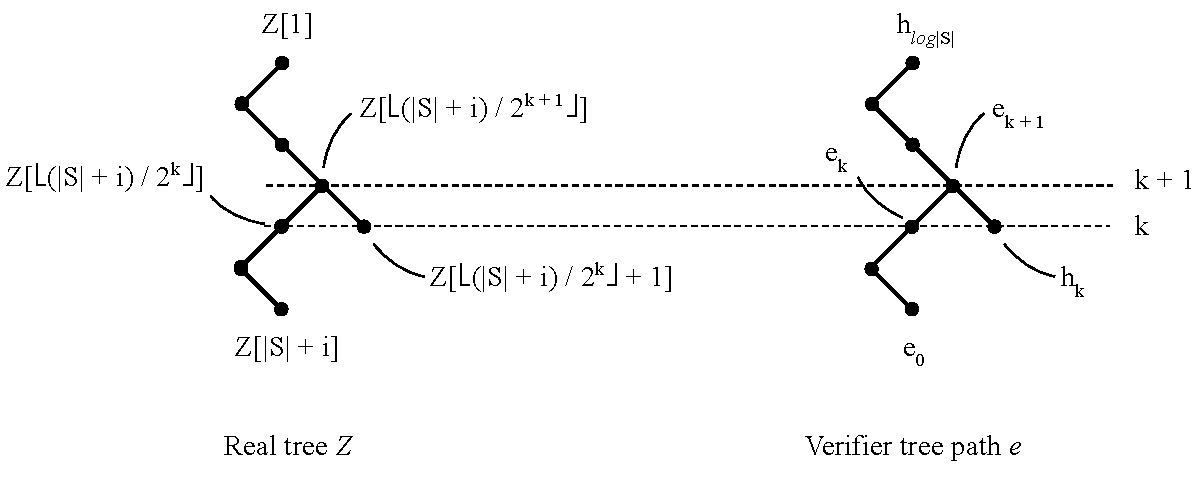
\includegraphics[width=\textwidth]{chapters/background/figures/mtpf.pdf}
  \caption{
    The path comparison between the real tree (left) $Z$ constructed using
    \textsf{heapify} and the verifier tree path (right) $h$ constructed by
    taking successive hashes with the sequence $s_i$ finds a collision at level
    $k$.
  }
  \label{fig.mtpf}
\end{figure}%}}}

The verifier who applies successive hashing will arrive at a
sequence of hashes $e_0, e_1, \cdots, e_{\log|S|}$. The
adversary $\mathcal{A}^*$ evaluates this sequence in the same manner as the
verifier would and also looks at the values $Z[|S| + i], Z[\lfloor \frac{|S| + 1}{2} \rfloor],
\cdots, Z[1]$ as obtained by $\textsc{heapify}(S)$. The adversary
$\mathcal{A}^*$ compares the two sequences and finds the minimum $k \geq 0$ such that
$Z[\lfloor \frac{|S| + i}{2^k} \rfloor] \neq e_k$, but
$Z[\lfloor \frac{|S| + i}{2^{k + 1}} \rfloor] = e_{k + 1}$. This is illustrated
in Figure~\ref{fig.mtpf}.
If $b_k = 0$,
then it returns the pair
$(Z[\lfloor \frac{|S| + i}{2^k} \rfloor] \concat Z[\lfloor \frac{|S| + i}{2^k} \rfloor + 1],\allowbreak e_k \concat h_k)$ as a
collision. If $b_k = 1$ it returns the pair
$(Z[\lfloor \frac{|S| + i}{2^k} \rfloor - 1]\concat Z[\lfloor \frac{|S| + i}{2^k} \rfloor],\allowbreak h_k \concat e_k)$. If no such $k$ is found, it aborts.

We argue that
$\Pr[\textsf{hash-collision}_{H,\mathcal{A}^*}] \geq
 \Pr[\textsf{auth}_{\Pi,\mathcal{A}}]$. To see this, consider the event that
$\mathcal{A}$ is successful. It suffices to show that $\mathcal{A}^*$ is also
successful. We distinguish two cases. In the first case,
we have $H(e) = H(S_i)$. As $e \neq S_i$, therefore $\mathcal{A}^*$ has
found a collision and the condition holds. Otherwise we have that
$H(e) \neq H(S_i)$. As the verification is successful, we must have $h_{\log|S|} = s$.
Therefore there must exist some $k$ at which the condition holds. Without loss
of generality, let $b_k = 0$.
As $Z[\lfloor \frac{|S| + i}{2^k} \rfloor] \neq e_k$ we have that
$Z[\lfloor \frac{|S| + i}{2^k} \rfloor] \concat h_k \neq e_k \concat h_k$.
Additionally,
$Z[\lfloor \frac{|S| + 1}{2^{k + 1}} \rfloor] = e_{k + 1} = \text{``h:''} \concat H(\lfloor Z[\frac{|S| + i}{2^k} \rfloor] \concat Z[\lfloor \frac{|S| + i}{2^k} \rfloor + 1]) = \text{``h:''} \concat H(e_k \concat h_k)$,
so a collision has occurred.

For the case $|\pi| < \log|S|$, the adversary $\mathcal{A}^*$ finds the
internal node of the tree $Z$ which lies at a distance $|\pi|$ from the root and
its index at this level is again constructed from the binary number obtained
by concatenating the bits $b$ in $\pi$. Since it is the internal node of a
complete tree, it has two children $a$ and $b$ and its value will be
$\text{``h:''} \concat H(a \concat b)$ where $a$ is also prefixed by ``h:''. On
the other hand, the claimed $e$ is prefixed by ``c:'', and so $e \neq a
\concat b$. The adversary $\mathcal{A}^*$ then proceeds to find the minimum
$k$ as before, but this time starting at a distance only $|\pi|$ from the root
instead of $\log|S|$.

Lastly, for the case $|\pi| > \log|S|$, the adversary
$\mathcal{A}^*$ applies $|\pi| - \log|S| - 1$ successive hashes with the sequence
$s_0,\allowbreak s_1,\allowbreak \cdots,\allowbreak s_{|\pi| - \log|S| - 1}$
on the sides
$b_0,\allowbreak b_1,\allowbreak \cdots,\allowbreak b_{|\pi| - \log|S| - 1}$
in the same manner that the verifier
would by consuming the first $|\pi| - \log|S| - 1$ elements of $\pi$. At that
point, it arrives at some value $v$ which is prefixed by ``h:''. It then
computes $i$ as before by using the remaining bits $b$ in the proof that has not
yet been consumed, and considers the element $S_i$ for which it will hold that
$v \neq S_i$ since it is prefixed by ``c:''. It can then proceed as before to
find $k$.
\end{proof}

Once the marking of nodes as leaves or internal nodes
has been established, the limitation that $|S| = 2^k$ can also be relaxed by
working with an incomplete binary tree instead of a complete binary tree.
